\begin{figure}[H]
	\center
	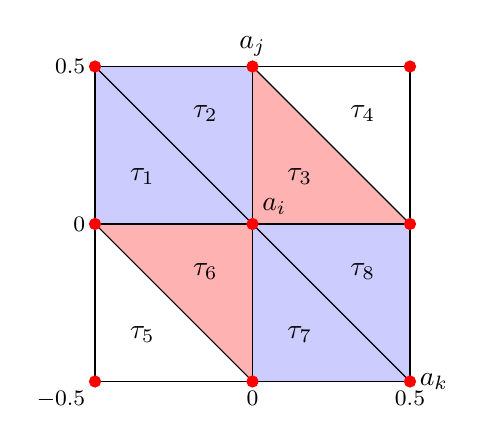
\begin{tikzpicture}[scale=2]
	
	\pgfmathsetmacro{\zerox}{-1}
	\pgfmathsetmacro{\zeroy}{-1}
	
	%color the important triangles
	\fill[red!30!] (\zerox,\zeroy) ++ (1,1) -- ++(0,-1) -- ++(-1,+1) --cycle;
	\fill[red!30!] (\zerox,\zeroy) ++ (1,1) -- ++(0,1) -- ++(1,-1) --cycle;
	
	\fill[blue!20!] (\zerox,\zeroy) ++ (1,1) -- ++(-1,0) -- ++(0,+1) -- ++(1,0) --cycle;
	\fill[blue!20!] (\zerox,\zeroy) ++ (1,1) -- ++(1,0) -- ++(0,-1) -- ++(-1,0) --cycle;
	
	% draw outline
	\draw (\zerox,\zeroy) -- ++(2,0)-- ++(0,2) --++(-2,0) --cycle;
	
	%vertical lines
	\draw (\zerox,\zeroy) ++(1,0)-- ++(0,2);
	
	% horizontal lines
	\draw (\zerox,\zeroy) ++(0,1)-- ++(2,0);

	
	% diagonal lines
	\draw (\zerox,\zeroy) ++(0,1)-- ++(1,-1);
	\draw (\zerox,\zeroy) ++(0,2)-- ++(2,-2);
	\draw (\zerox,\zeroy) ++(1,2)-- ++(1,-1);
	
	
	% inner points
	\filldraw[red]  (\zerox,\zeroy) circle (1pt)
					(\zerox,\zeroy) ++ (0,1) circle (1pt)
					(\zerox,\zeroy) ++ (0,2) circle (1pt)
					(\zerox,\zeroy) ++ (1,0) circle (1pt)
					(\zerox,\zeroy) ++ (1,1) circle (1pt)
					(\zerox,\zeroy) ++ (1,2) circle (1pt)
					(\zerox,\zeroy) ++ (2,0) circle (1pt)
					(\zerox,\zeroy) ++ (2,1) circle (1pt)
					(\zerox,\zeroy) ++ (2,2) circle (1pt);
	
	
	% number triangles
	\fill[black] (\zerox,\zeroy) ++ (0.3,1.3) node[] {$\tau_1$}
				 (\zerox,\zeroy) ++ (0.7,1.7)  node[] {$\tau_2$}
				 (\zerox,\zeroy) ++ (1.3,1.3)  node[] {$\tau_3$}
				 (\zerox,\zeroy) ++ (1.7,1.7)  node[] {$\tau_4$}
				 (\zerox,\zeroy) ++ (0.3,0.3)  node[] {$\tau_5$}
				 (\zerox,\zeroy) ++ (0.7,0.7)  node[] {$\tau_6$}
				 (\zerox,\zeroy) ++ (1.3,0.3)  node[] {$\tau_7$}
				 (\zerox,\zeroy) ++ (1.7,0.7)  node[] {$\tau_8$};

	
	
	% axis numbering
	\fill[black,font=\footnotesize] (\zerox,\zeroy)  node[below left] {$-0.5$}
									(\zerox,\zeroy) ++(1,0) node[below] {$0$}
									(\zerox,\zeroy) ++(2,0) node[below] {$0.5$}
									
									(\zerox,\zeroy) ++(0,1) node[left] {$0$}
									(\zerox,\zeroy) ++(0,2) node[left] {$0.5$};
									
	\fill[black] (\zerox,\zeroy) ++(1,1)  node[above right] {$a_i$}
				 (\zerox,\zeroy) ++(1,2)  node[above] {$a_j$}
   				 (\zerox,\zeroy) ++(2,0)  node[right] {$a_k$};

	
	\end{tikzpicture}
		
	\caption{important $\tau $}\label{tikz/chapter2/important_tau}
	\label{ch2_important_tau}

\end{figure}